In this section, we evaluate the performance of different synchronization protocols in \textit{dxex}.
We also compare to \textit{adevs}~\cite{adevs}, currently one of the most efficient simulation kernels~\cite{DEVStoneJournal}, to show that our modularity does not impede performance.
CPU time and memory usage is compared for both sequential and parallel simulation.

We start off with a comparison of sequential simulation, to show how \textit{adevs} and \textit{dxex} relate in this simple case.
For the parallel simulation benchmarks, results are presented for both conservative and optimistic synchronization.

For all benchmarks, results are well within a 5\% deviation of the average, such that only the average is used in the remainder of this section.
The same compilation flags were used for both \textit{adevs} and \textit{dxex} benchmarks (``\texttt{-O3 -flto}'').
To guarantee comparable results, no I/O was performed during benchmarks.
Before benchmarking, simulation traces were used to verify that \textit{adevs} and \textit{dxex} return exactly the same simulation results.
Benchmarks were performed using Linux, but our simulation tool works equally well on Windows and Mac.
The exact parameters for each benchmark can be found in our repository. 

The benchmarks are ran on a machine with 8 x AMD Opteron(TM) Processor 6274 with 8 cores per CPU (for a total of 64 cores) and 192 GB RAM.

\subsection{Benchmark Models}
We use three different benchmark models, covering different aspects of the simulation kernel.

First, the \textit{Queue} model, based on the \textit{HI} model of DEVStone~\cite{DEVStone}, creates a chain of hierarchically nested atomic \textsf{DEVS} models.
A single generator pushes events into the queue, which get consumed by the processors after a fixed or random delay.
It takes two parameters: the width and depth of the hierarchy.
This benchmark shows how the complexity of the simulation kernel behaves for an increasing amount of atomic models, and an increasingly deep hierarchy.
An example for a width and depth of 2 is shown in Figure~\ref{fig:queue_model}.
	
Second, the \textit{Interconnect} model, a merge of PHOLD~\cite{PHOLD} and the \textit{HI} model of DEVStone~\cite{DEVStone}, creates $n$ atomic models, where each model has exactly one output port.
Similar to PHOLD, all models are connected to one another, but all through the same port: every model receives each generated event (\textit{i.e.}, the event is broadcasted).
The model takes one parameter: the number of models.
This benchmark shows the complexity of event creation, event routing, and simultaneous event handling.
An example for three models is shown in Figure~\ref{fig:interconnect_model}.

Third, the \textit{PHOLD} model~\cite{PHOLD}, creates $n$ atomic models, where each model has exactly $n-1$ output ports.
Each atomic model is directly connected to every other atomic model.
After a random delay, an atomic model sends out an event to a randomly selected output port.
Output port selection happens in two phases: first it is decided whether the event should be sent within the same node, or outside of the node.
Afterwards, a uniform selection is made between the remaining models.
The model takes two parameters: the percentage of remote events (determining the percentage of messages routed to other nodes), and the percentage of high-priority events.
High-priority events are events generated in a very short time after the previous event.
This benchmark shows how the simulation kernel behaves in the presence of many local or remote events, in combination with a varying percentage of high-priority events.
An example for four models, split over two nodes, is shown in Figure~\ref{fig:PHOLD_model}.

\begin{figure}
	\center
	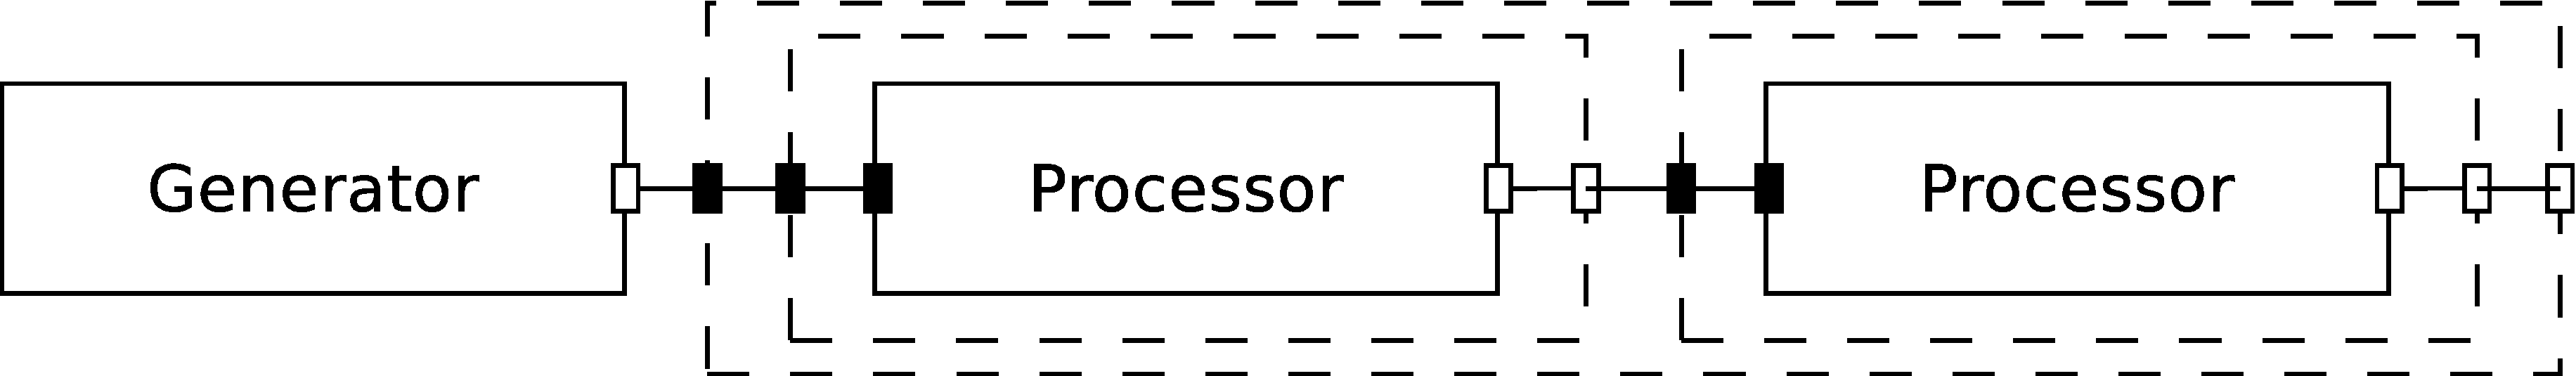
\includegraphics[width=\columnwidth]{fig/queue_model_fixed.pdf}
	\caption{Queue model for depth and width 2.}
	\label{fig:queue_model}
\end{figure}
	
\begin{figure}
    \center
	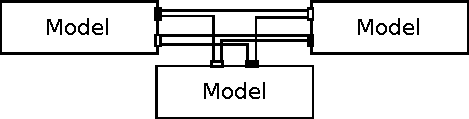
\includegraphics[width=\modelfraction\columnwidth]{fig/interconnect_model.pdf}
	\caption{Interconnect model for three models.}
	\label{fig:interconnect_model}
\end{figure}

\begin{figure}
    \center
	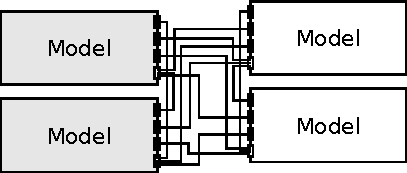
\includegraphics[width=\modelfraction\columnwidth]{fig/phold_model.pdf}
	\caption{PHOLD model for three models.}
	\label{fig:PHOLD_model}
\end{figure}

\subsection{Sequential Simulation}
We start by evaluating sequential simulation performance, in order to obtain a baseline for our comparison of parallel simulation performance.

\subsubsection{Queue}
\label{4-seq-Queue}
For the first benchmark, we tested the effect of hierarchical complexity of the model in the performance of the simulator.
A set of three tests was performed, where each test has the same number of models but an increasing depth.
The results can be seen in Figure~\ref{fig:Queue_benchmark_seq}.
Since \textit{dxex} performs direct connection~\cite{SymbolicFlattening} on the model, there is no performance hit when the depth is increased.
Direct connection only needs to be done at initialization, so it is a one time cost that is negligible for long running simulations.
\textit{Adevs}, on the other hand, suffers from the increased depth, even though some similar (but not identical) optimization to event passing was made~\cite{adevs_opt}.
With every new hierarchical layer, routing an event from one atomic model to the next becomes more expensive, resulting in an increase in runtime.

\begin{figure}
	\center
	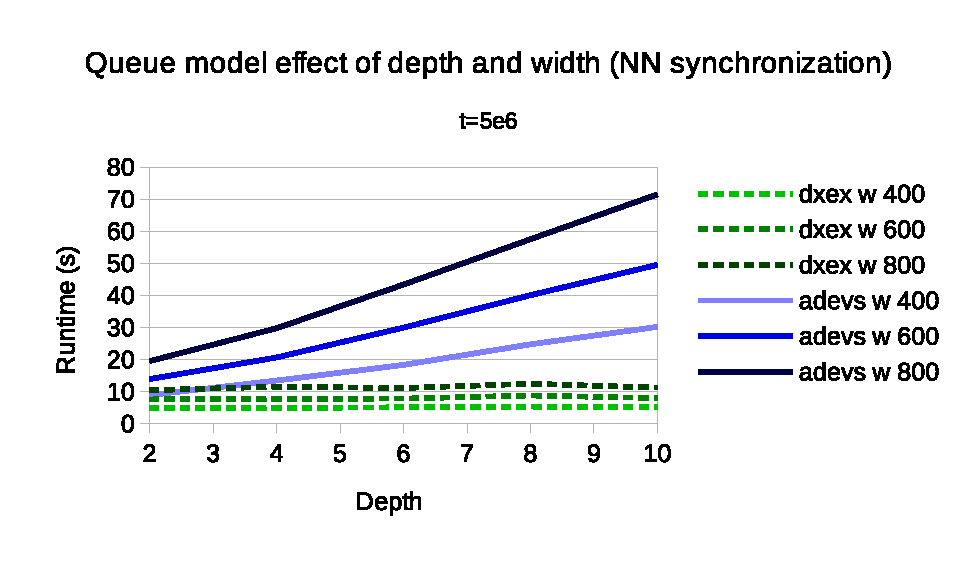
\includegraphics[width=\columnwidth]{fig/queue_fixed_sequential.eps}
	\caption{Queue benchmark results for sequential simulation.}
	\label{fig:Queue_benchmark_seq}
\end{figure}

\subsubsection{Interconnect}
\label{4-seq-Interconnect}
In the Interconnect model, we increase the number of atomic models, quadratically increasing the number of couplings and the number of external transitions.
As shown in Figure~\ref{fig:Interconnect_benchmark}, \textit{adevs} now outperforms \textit{dxex} by a fair margin.
Analysis showed that this is caused by the high amount of events: event creation is much slower in \textit{dxex} than it is in \textit{adevs}, despite \textit{dxex}'s use of memory pools.
To shield the user from threading and deallocation concerns \textit{dxex} provides an event superclass from which the user can derive to create a specialized event type.
Copying, deallocation, and tracing are done at runtime, adding significant overhead when events happen frequently.
Profiling the benchmarks revealed the increased cost of output generation and deallocation as the determining factor.

\begin{figure}
	\center
	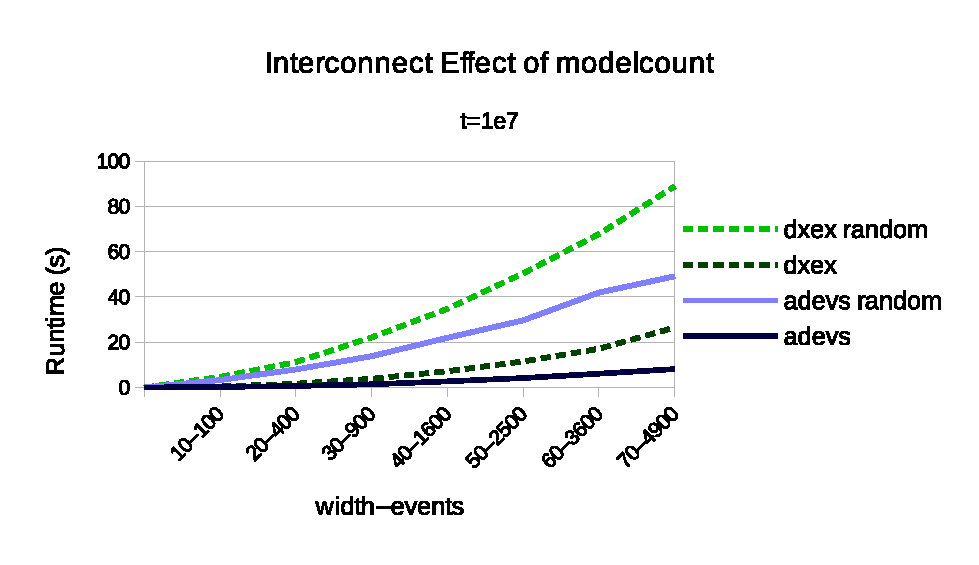
\includegraphics[width=\columnwidth]{fig/interconnect_sequential.eps}
	\caption{Interconnect benchmark results for sequential simulation.}
	\label{fig:Interconnect_benchmark}
\end{figure}

\subsubsection{PHold}
\label{4-seq-PHold}
The PHold model is very similar to the Interconnect model.
The biggest difference is that the amount of messages sent is much lower.
The number of events scales linear with the number of models, not quadratic.
Figure~\ref{fig:Phold_benchmark} shows that the performance of \textit{dxex} and \textit{adevs} are very close to each-other, with \textit{adevs} slightly outperforming \textit{dxex}.

\begin{figure}
	\center
	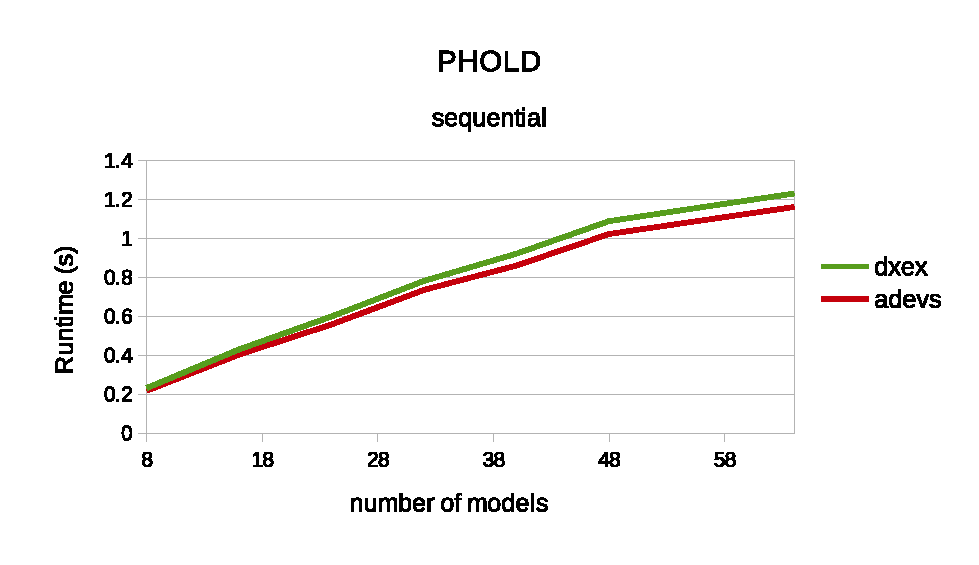
\includegraphics[width=\columnwidth]{fig/phold_sequential.eps}
	\caption{PHold benchmark results for sequential simulation.}
	\label{fig:Phold_benchmark}
\end{figure}

\subsection{Parallel Simulation}
We now continue by describing our parallel simulation performance for different synchronization protocols, and compared to \textit{adevs}.
The speedup of \textit{adevs} is computed with the corresponding \textit{dxex} sequential benchmark.
This was done to take into account the performance difference observed in sequential simulation.
As such, the highest speedup indicates the fastest results among all tools, independent of sequential simulation results.

\subsubsection{Queue}
The Queue model is one single chain of models, resembling a pipeline.
This structure can be exploited to prevent cyclic dependencies in the parallel simulation.

Figure~\ref{fig:Queue_plot_strong} shows the speedup compared to sequential simulation for a fixed problem size (\textit{i.e.}, strong scaling).
As the number of kernels increases, the optimistic kernel quickly becomes the worst choice.
This is mainly caused by the pipeline structure of the model: the last models in the queue only respond to incoming messages and therefore have to be rolled back frequently.
The difference between \textit{dxex} conservative and \textit{adevs} becoms smaller when more and more cores are used.
The same effect can be seen when the problem size is increased in tandem with the number of used cores (\textit{i.e.}, weak scaling) in Figure~\ref{fig:Queue_plot_weak}.

\begin{figure}
	\center
	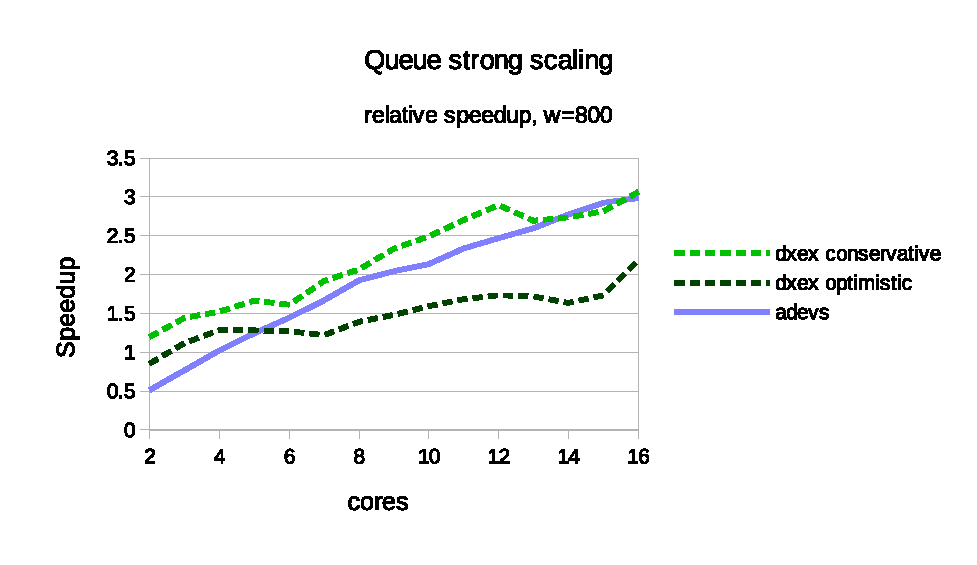
\includegraphics[width=\columnwidth]{fig/queue_fixed_strong_speedup.eps}
	\caption{Queue model strong scaling speedup compared to \textit{dxex} sequential.}
	\label{fig:Queue_plot_strong}
\end{figure}

\begin{figure}
	\center
	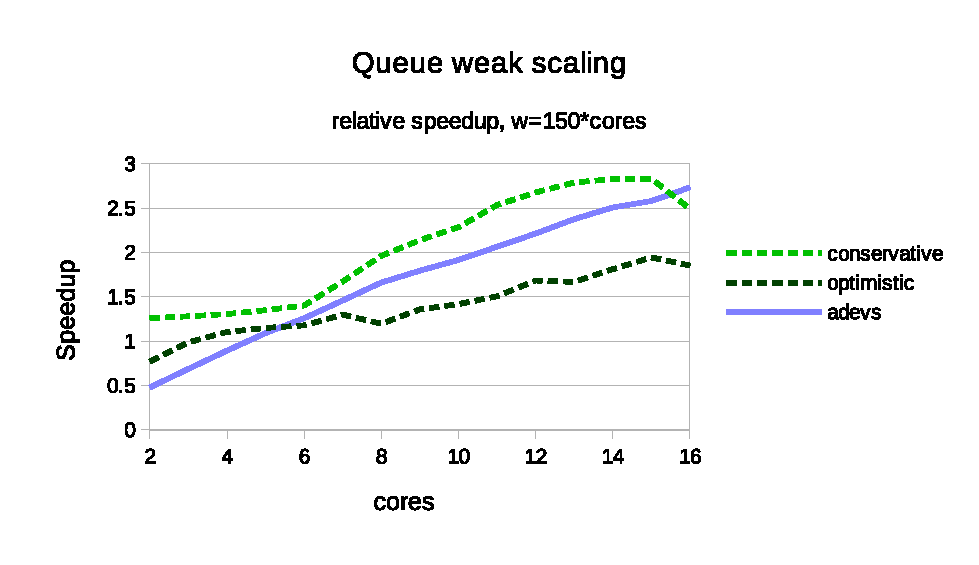
\includegraphics[width=\columnwidth]{fig/queue_fixed_weak_speedup.eps}
	\caption{Queue model weak scaling speedup compared to \textit{dxex} sequential.}
	\label{fig:Queue_plot_weak}
\end{figure}
	
\subsubsection{Interconnect}
\label{subsec:parallelinterconnect}
In the Interconnect model, we determine how broadcast communication is supported across multiple nodes.
The number of models is now kept constant at eight.
Results are shown in Figure~\ref{fig:interconnect_benchmark_parallel}.
When the number of nodes increases, performance decreases due to increasing contention in conservative simulation and the increasing number of rollbacks in optimistic simulation.
All models depend on each other and have no computational load whatsoever, negating any possible performance gain by executing the simulation in parallel.

\begin{figure}
	\center
	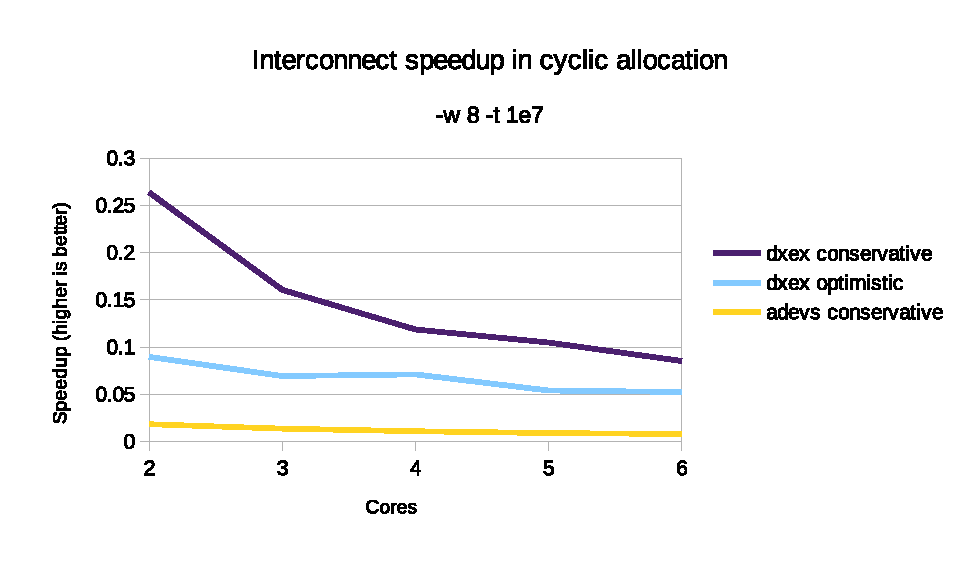
\includegraphics[width=\columnwidth]{fig/interconnect_parallel.eps}
    %TODO cyclic allocation in title?
	\caption{Interconnect benchmark results for parallel simulation.}
	\label{fig:interconnect_benchmark_parallel}
\end{figure}

\subsubsection{PHOLD}
In the PHOLD model, we first investigate the influence of the percentage of remote events on the speedup.
A remote event in this context is an event that is sent from a model on one kernel to a model on another simulation kernel.
When remote events are rare, optimistic synchronization rarely has to roll back, thus increasing performance.
With more frequent remote events, however, optimistic synchronization quickly slows down due to frequent rollbacks.
Conservative synchronization, on the other hand, is mostly unconcerned with the number of remote events: the mere fact that a remote event can happen, causes it to block and wait.
Even though a single synchronization protocol is always ideal in this case, it already shows that different synchronization protocols respond differently to a changing model.

\textit{Adevs} is significantly slower during conservative synchronization.
Analysis of profiling callgraphs shows that exception handling in \textit{adevs} is the main cause. 
To keep the models equivalent, the \textit{adevs} version does not provide the \{begin,end\}Lookahead methods, which accounts for the exception handling.
These functions require the user to implement a state saving method.
But in contrast to \textit{PythonPDEVS} and \textit{dxex}, which handle this inside the kernel, users need to manually define this.
We feel this would lead to an unfair comparison as we would like to keep the models agnostic of the underlying protocols across all benchmarks.

\begin{figure}
    \center
    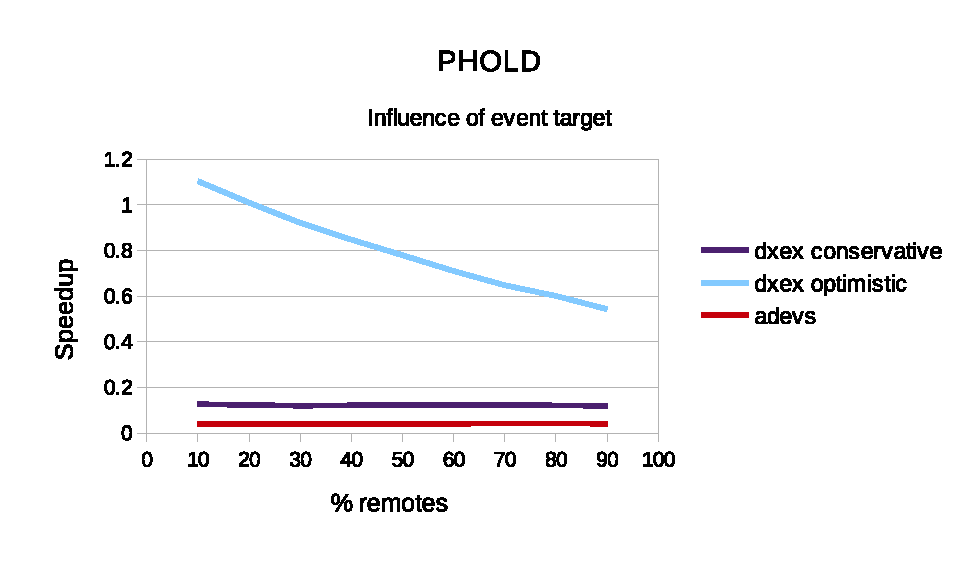
\includegraphics[width=\columnwidth]{fig/phold_remotes.eps}
    \caption{PHOLD benchmark results for parallel simulation using four kernels, with varying percentage of remote events.}
\end{figure}

\begin{figure}
	\center
	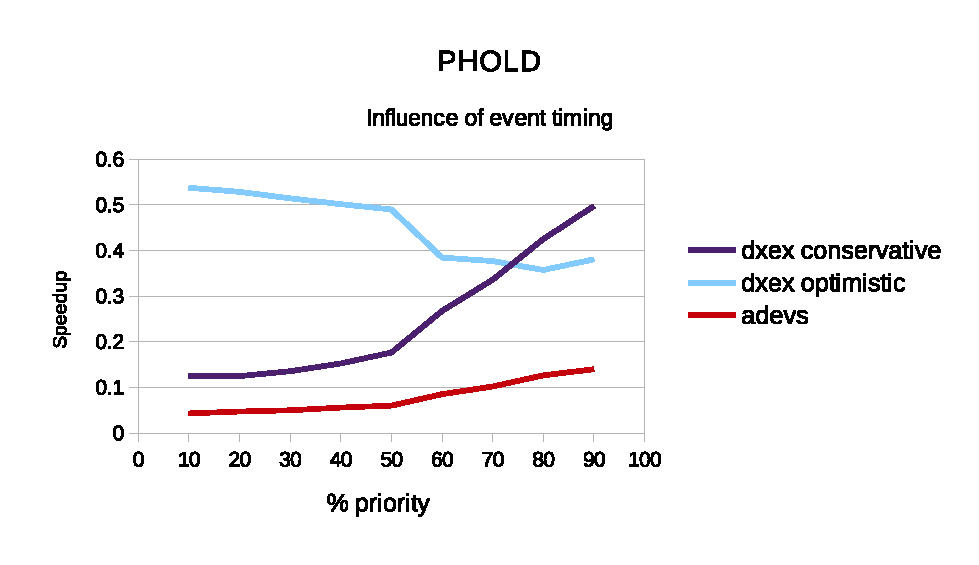
\includegraphics[width=\columnwidth]{fig/phold_priority.eps}
	\caption{PHOLD benchmark results for parallel simulation using four kernels, with varying amount of high-priority events.}
	\label{fig:phold_priority}
\end{figure}

Contrary to normal events, high-priority events happen almost instantaneously, restricting lookahead to a very small value.
Even when normal events occur most often, conservative synchronization always blocks until it can make guarantees.
Optimistic synchronization, however, simply goes forward in simulation time and rolls back when these high-priority events happen.
This situation closely mimics the model typically used for comparing conservative and optimistic synchronization~\cite{FujimotoBook}.

Figure~\ref{fig:phold_priority} shows how simulation performance is influenced by the fraction of these high-priority events.
If barely any high-priority events occur, conservative synchronization is penalized due to its excessive blocking, which often turned out to be unnecessary.
When many high-priority events occur, optimistic synchronization is penalized due to its unconditional progression of simulation, which frequently needs to be rolled back.
Results show that there is no single perfect synchronization algorithm for this kind of models: depending on configuration, either synchronization protocol might be better.

\subsection{Comparison to the abstract simulator}
The abstract simulator of \textsf{Parallel DEVS} included its own notion of parallelism: transition functions that happen at the same point in simulated time can be trivially parallelized.
This parallelization is trivial, in the sense that there is no need for synchronization protocols.
The parallelization of the transition functions (from now on called the ``inherent parallelism'') is, at least in \textit{dxex}, independent of the use of a synchronization protocol.
That is, both can be used simultaneously.
Following the theoretical analysis published in~\cite{amdahlpdevs}, a comparison between this inherent parallelism and the use of synchronization protocols is warranted.

\paragraph{Model}
We have opted to use the \textit{Queue} model for this comparison, as it allows for many interesting configurations.
%TODO what is meant with this allocation of threads and synchronized kernels?
The effect of combining 4 synchronized kernels, with each 4 threads for PDEVS, is contrasted with 16 threads for PDEVS and 16 kernels for conservative and optimistic.
This allows us to observe which is more efficient in obtaining a speedup.
We simulate a computational load by an optional call to sleep in the transition functions set at 5 milliseconds.
The model is configured with depth 4 and width 300 if the transition function has no load, and width 50 if the computational load is active.
In our configuration, an imminent model generates output, resulting in another model becoming imminent.
With respect to the theoretical analysis in~\cite{amdahlpdevs} this gives a parameter value $q = 1$.
Models are equally distributed over the kernels and between threads in PDEVS.
The coefficient of variation of our results is less than 1\%.
The communication overhead is hard to estimate, but given our coefficient of variation, we can expect this overhead to be constant.

We consider two cases: one where all transition functions happen simultaneously, and one where transition functions never happen simultaneously.
We defer the discussion on which of these two is the most realistic, as this depends on the problem domain.
For example, in a simulation with a fixed timestep (\textit{e.g.}, cell-based models, discretization of continuous model), transition functions will often occur simultaneously.
Conversely, simulations with an arbitrary timestep (\textit{e.g.}, many independent systems communicating together) have very few simultaneous events.

\paragraph{Concurrent events}
First we create a model where all transitions happen simultaneously, with a significant computational load in the transition functions.
In Figure~\ref{fig:pdevs_plot_fixed_sleep}, we observe that exploiting only the inherent parallelism, results in a speedup of about 10.  
%TODO again: what is this?
Simulation with conservative and optimistic synchronization is run first with 16 kernels, then with 4 kernels having 4 PDEVS threads each. 
Both synchronization protocols achieve a speedup similar to only exploiting the inherent parallelism.
Combining the protocols with the inherent parallelism gives near identical results.
In this scenario there is no real advantage between the different parallel configurations.

\begin{figure}
	\center
	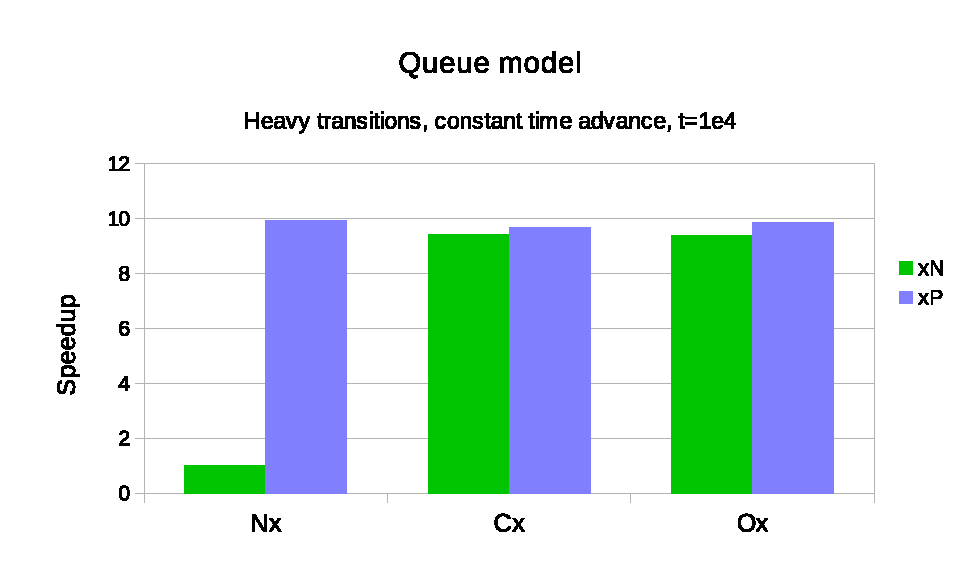
\includegraphics[width=\columnwidth]{fig/pdevs_fixed_sleep.eps}
    %TODO fix key in figure: pdevs --> inherent parallelism
	\caption{Queue speedup benchmark for PDEVS and synchronization with maximal concurrent events and significant computational load}
	\label{fig:pdevs_plot_fixed_sleep}
\end{figure}

\paragraph{Random events}
Now we randomize the time advance in the models, resulting in very few transition functions that happen simultaneously.
Even when two transitions are only minimally apart in simulated time, they cannot be executed in parallel, as there might otherwise be a causality error.
The transition function has the same computational load as in the previous configuration. 
The results in Figure~\ref{fig:pdevs_plot_random_sleep} show that parallelizing transition functions only, adds little overhead. 
Nonetheless, performance is not increased at all: the chances of executing a few transition functions in parallel does not make up for the overhead of checking.
In combination with either synchronization protocol, a minor improvement can still be seen, but this is primarily caused by the synchronization protocol, and not by parallelizing the transition functions.

\begin{figure}
	\center
	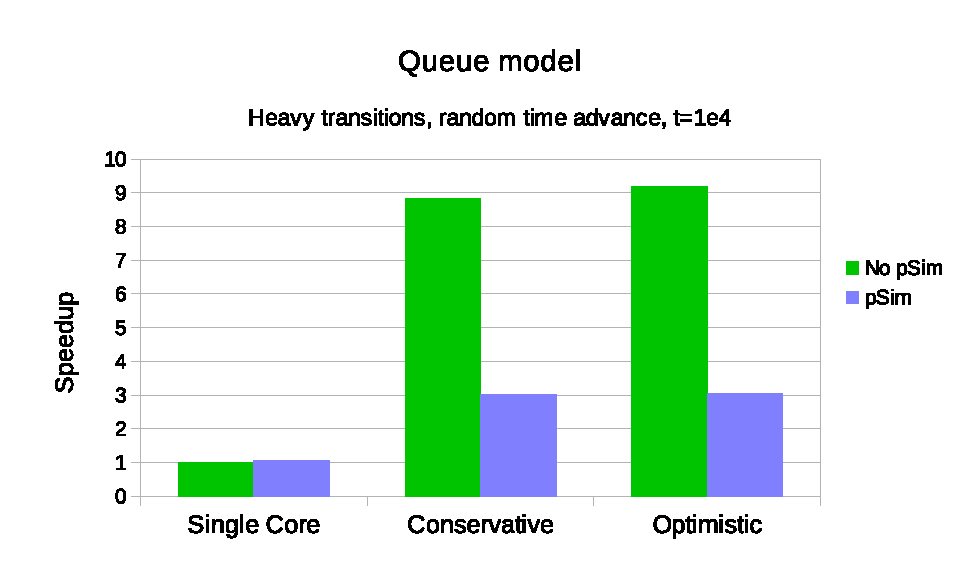
\includegraphics[width=\columnwidth]{fig/pdevs_random_sleep.eps}
    %TODO fix key in figure: pdevs --> inherent parallelism
	\caption{Queue speedup benchmark for PDEVS and synchronization with randomized events and significant computational load}
	\label{fig:pdevs_plot_random_sleep}
\end{figure}

\paragraph{Computational load}
Finally, we remove the computation load from the transition function, in combination with many concurrent events.
Figure~\ref{fig:pdevs_plot_no_sleep} shows that in sequential simulation, the overhead of thread management and shared memory communication is crippling for performance.
Even though many events occur concurrently, the actual computation being done in the transition function does not outweight the overhead, resulting in much slower simulation than sequential execution of transition functions.
When combined with synchronization protocols, performance is still reasonable, though the use of the inherent parallelism is not beneficial either way.
Both synchronization protocols achieve a reasonable speedup without PDEVS, as the overhead of thread management (creation and destruction) is avoided.
These results are similar to~\cite{Himmelspach}.
 
\begin{figure}
	\center
	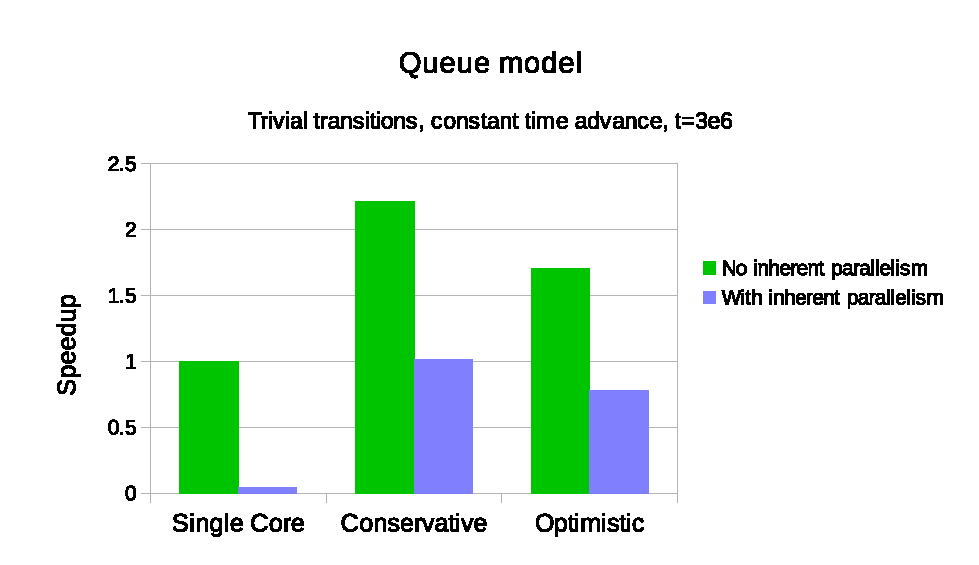
\includegraphics[width=\columnwidth]{fig/pdevs_no_sleep.eps}
    %TODO fix key in figure: pdevs --> inherent parallelism
	\caption{Queue speedup benchmark for PDEVS and synchronization with maximal concurrent events and trivial computational load}
	\label{fig:pdevs_plot_no_sleep}
\end{figure}

\paragraph{Discussion}
In \textit{dxex}, use of the inherent parallelism found in \textsf{Parallel DEVS} can be combined with any of the supported synchronization protocols.
The user is not forced to choose between either but can divide the capabilities of his machine over both approaches.
While exploitation of the inherent parallelism can offer a significant speedup, a high number of transitions must be triggered simultaneously throughout the whole simulation.
Additionally, the computational load of the transition functions should be high enough to warrant the thread management overhead.
We conclude that both approaches have their distinct advantages and disadvantages.
The inherent parallelism of \textsf{Parallel DEVS} avoids synchronization overhead and is trivial to implement.
It is not influenced by the coupling of models, and only by the number of simultaneous transition functions and the computational load in the transition function.
In contrast, either of the two synchronization protocols is heavily influenced by the coupling of the models, but not by the computational load or number of simultaneous transitions.

\subsection{Memory Usage}
Apart from simulation execution time, memory usage during simulation is also of great importance.
While execution time only becomes a problem if it takes way too long, coming short only a bit of memory can make simulation infeasible.
We therefore also investigate the memory usage of different synchronization protocols, and again compare to \textit{adevs}.

We do not tackle the problem of states that become too large for a single machine to hold.
This problem can be mitigated by distribution over multiple machines, which neither \textit{dxex} or \textit{adevs} support.

\subsubsection{Remarks}
Both \textit{dxex} and \textit{adevs} use \textit{tcmalloc} as memory allocator, allowing for thread-local allocation.
Additionally, dxex uses memory pools to further reduce the frequency of expensive system calls (\textit{e.g.}, malloc and free).
\textit{tcmalloc} only gradually releases memory back to the OS, whereas our pools will not do so at all.
Due to our motivation for memory usage analysis, we will only measure peak allocation in maximum resident set size as reported by the OS.

\subsubsection{Results}
Figure~\ref{fig:memory} shows the memory used by the different benchmarks.
Results are in megabytes, and show the total memory footprint of the running application (\textit{i.e.}, text, stack, and heap).
Note the logarithmic scale due to the high memory consumption of optimistic synchronization.

Unsurprisingly, optimistic synchronization results show very high memory usage due to the saved states.
Note the logarithmic scale that was used for this reason.
Optimistic synchronization results vary heavily depending on thread scheduling by the operating system, as this influences the drift between nodes. 
Comparing similar approaches, we notice that \textit{dxex} and \textit{adevs} have very similar memory use.

Conservative simulation always uses more memory than sequential simulation, as is to be expected.
Additional memory is required for the multiple threads, but also to store all events that are processed simultaneously.

\begin{figure}
    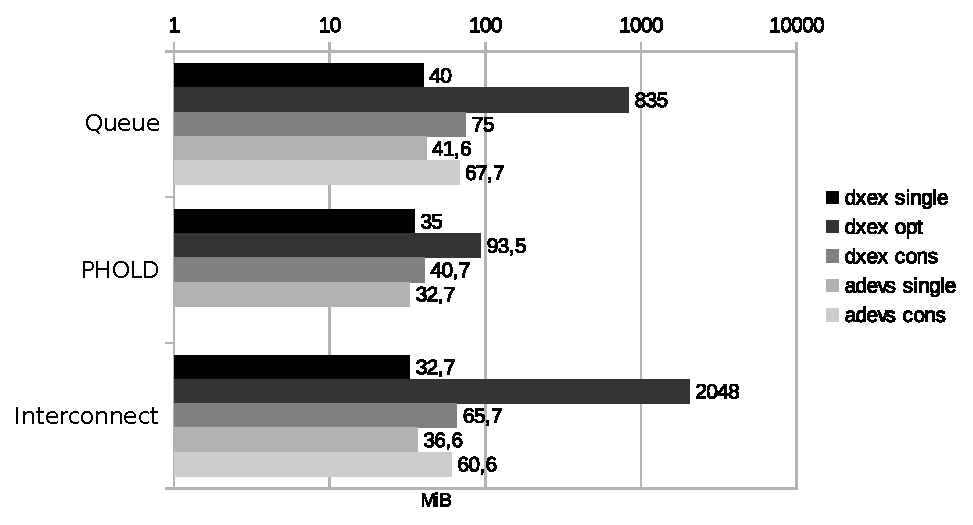
\includegraphics[width=\columnwidth]{fig/memory_voorlopig.eps}
    \caption{Memory usage results.}
    \label{fig:memory}
\end{figure}

\subsection{Conclusions on Performance Evaluation}
We have shown that our contribution is invaluable for high performance simulation: depending on the expected behaviour, modellers can choose the most appropriate synchronization protocol.
The use of synchronization protocols does also not prevent the exploitation of the inherent parallelism found in \textsf{ParallelPDEVS}.
Both approaches are useful in specific model configurations.
But even with the right synchronization protocol, we have seen that two problems remain.

First, although one of both synchronization protocols might be ideally suited for specific model behaviour, nothing guarantees that the model will exhibit the same behaviour throughout the simulation.
Similarly to the polymorphic scheduler~\cite{MasterThesis}, we wish to make it possible for the ideal option to be switched during simulation.
When changes to the model behaviour are noticed, the used synchronization protocol can be switched as well. 

Second, the allocation of models is nontrivial and has a significant impact on performance.
While our parallel speedup for the Queue model, for example, was rather high, this is mostly due to characteristics of the model: the dependency graph does not contain any cycles.
When cycles were introduced, as in the Interconnect model, performance became disastrous.

In the next two sections, we elaborate on these two problems.
